
% vim:set ff=unix expandtab ts=2 sw=2:
  {\vspace{.2cm}\textbf{REddyProc}\hfill\normalsize{A. Moffat, T. Wutzler, O. Menzer \& M. Migliavacca}}
\alert{\textit{Context:}}

\begin{itemize}
    \item Data from eddy covariance measurements are key to understand atmosphere ecosystem exchange fluxes.
    \item A standardized processing of the raw data is necessary to ensure comparability across sites.
    \item Site PIs will benefit from being able to process their data by using the easy-to-use R-package.
\end{itemize}
 

\begin{columns}
\column{.8\textwidth}
    \begin{figure}[tb]
    \begin{center}
        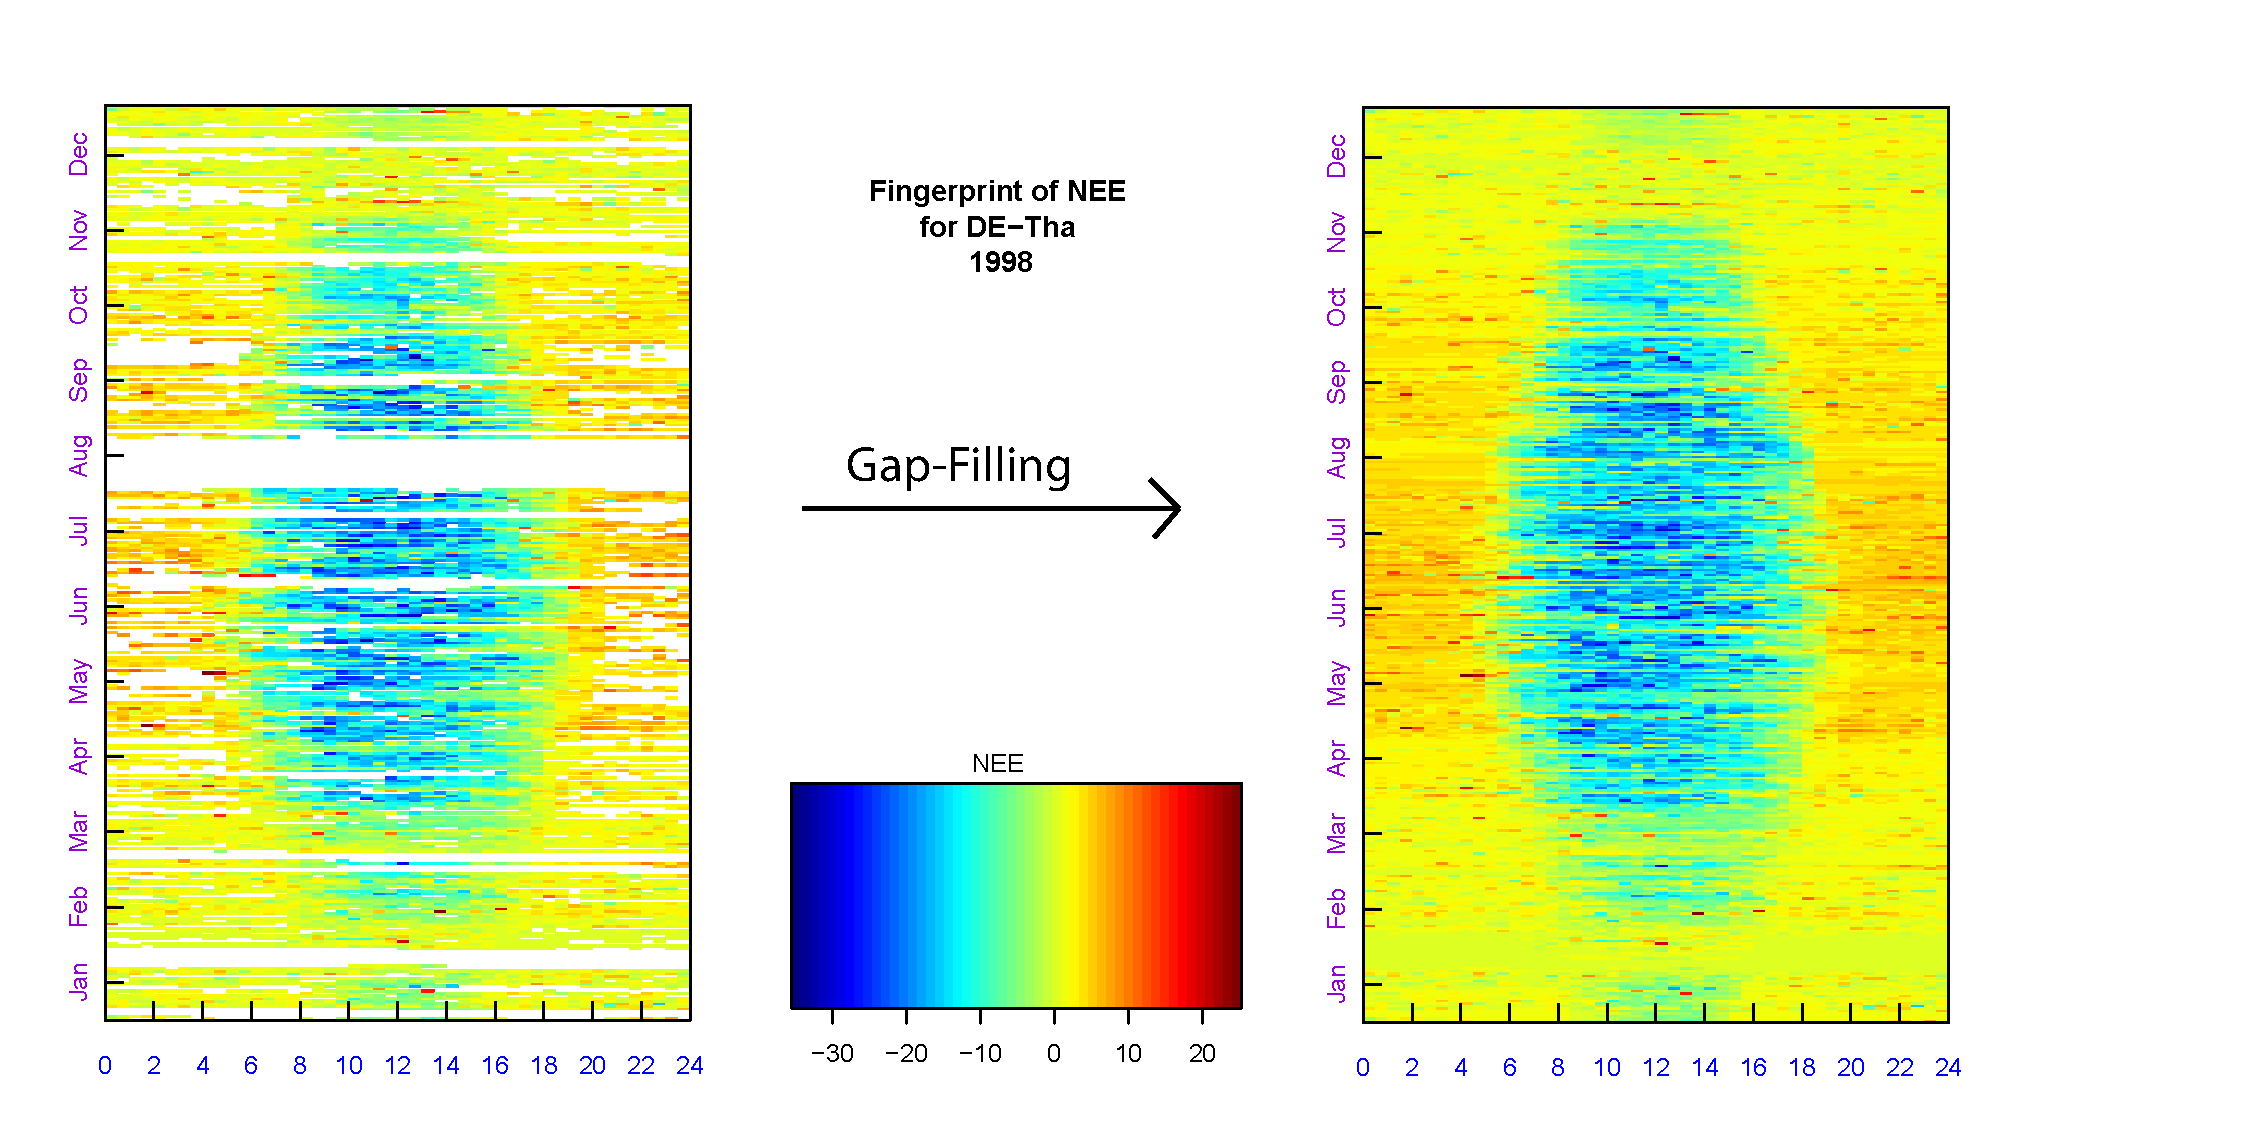
\includegraphics[width=.95\textwidth]{images/content/DE-Tha_1998_FP_NEE_ffc}
    \end{center}
    \end{figure}
\column{.2\textwidth}
\small{\textit{A fingerprint of ecosystem: Net ecosystem exchange (NEE) versus daytime and yearday}}
\vspace{4cm}
	\begin{figure}[tb]
		
\includegraphics[width=.6\textwidth]{images/qrcodeREddyProc.jpg}
	\end{figure}
\end{columns}
\vspace{1cm}
\hfill\large{\url{https://www.bgc-jena.mpg.de/bgi/index.php/Services/REddyProcWeb}}
